% @Author: AnthonyKenny98
% @Date:   2020-02-22 15:53:59
% @Last Modified by:   AnthonyKenny98
% @Last Modified time: 2020-02-27 15:46:33

\ac{RRT} is an algorithm designed to efficiently search, and thus plan a path through, a high-complexity environment by randomly sampling points and building a tree. The algorithm randomly samples points, draws an edge from the nearest currently existing node in the tree, to grow the tree in the space. It is inherently biased to grow towards large unsearched areas of the problem. RRT was developed by S. LaVelle\cite{LaValle1998} and J. Kuffner\cite{LaValle2001}. It is used in autonomous robotic motion planning problems such as autonomous drones, the focus of this thesis.

\subsection{Algorithm}

    The pseudocode for \ac{RRT} can be seen in Algorithm \ref{algorithm:rrt}
    % @Author: AnthonyKenny98
% @Date:   2020-02-27 10:55:29
% @Last Modified by:   AnthonyKenny98
% @Last Modified time: 2020-02-27 15:45:23

\begin{algorithm}[H]
    \caption{Rapidly-Exploring Random Tree in Free Configuration Space}
    \SetAlgoLined
    \SetArgSty{textnormal}
    \begin{tabular}{l l}
    \textbf{Inputs:}    & Initial configuration $q_{init}$,\\ 
                        & Number of nodes in graph $K$, \\
                        & Incremental Distance $\Delta q$ \\
    \textbf{Output:}    & RRT Graph $G$ with $K$ configurations \& edges \\
    \end{tabular}

        $G$.init()\;
        \For{$k = 1$ to $K$}{
            $q_{rand} \leftarrow $ randomConfiguration(); \\
            $q_{near} \leftarrow $ nearestVertex($q_{rand}$, $G$); \\
            $q_{new} \leftarrow $ newVertex($q_{near}$, $q_{rand}$, $\Delta q$); \\
            $G$.addVertex($q_{new}$); \\  
            $G$.addEdge($q_{near}$, $q_{new}$);
        }
\label{algorithm:rrt}
\end{algorithm}

    \todo[inline]{Explanation of RRT and how it relates to configuration}
    Algorithm \ref{algorithm:rrt} can be visually represented in Figure \ref{fig:rrt-step-by-step}. Consider a \ac{2D} robot operating in a \ac{2D} workspace. A Graph $G$ is initialized containing an initial configuration, $q_{init}$, with constraints on the number of nodes that the graph can hold, $K$, and the maximum distance between two nodes, $\Delta q$. This is shown in Subfigure \ref{subfig:rrt-step-by-step-A}. A random configuration for the robot, $q_{rand}$ is generated (\ref{subfig:rrt-step-by-step-B}). The nearest existing configuration in $G$, $q_{near}$, is found. (In the first iteration, $q_{near} = q_{init}$, shown in Subfigure \ref{subfig:rrt-step-by-step-C}). The distance between $q_{near}$ and $q_{rand}$ is calculated. If this distance is less than $\Delta q$, $q_{new} = q_{rand}$. If not, $q_{new}$ is selected, typically by moving by $\Delta q$ from $q_{near}$ towards $q_{rand}$ (\ref{subfig:rrt-step-by-step-C}). $q_{new}$ is then added to $G$. This is repeated for $K$ configurations.

    % @Author: AnthonyKenny98
% @Date:   2020-02-27 14:22:10
% @Last Modified by:   AnthonyKenny98
% @Last Modified time: 2020-02-27 15:36:30

\begin{figure}[H]
\begin{center}
\begin{tabular}{c c}

    % Subfigure A
    \begin{subfigure}{0.45\textwidth}
    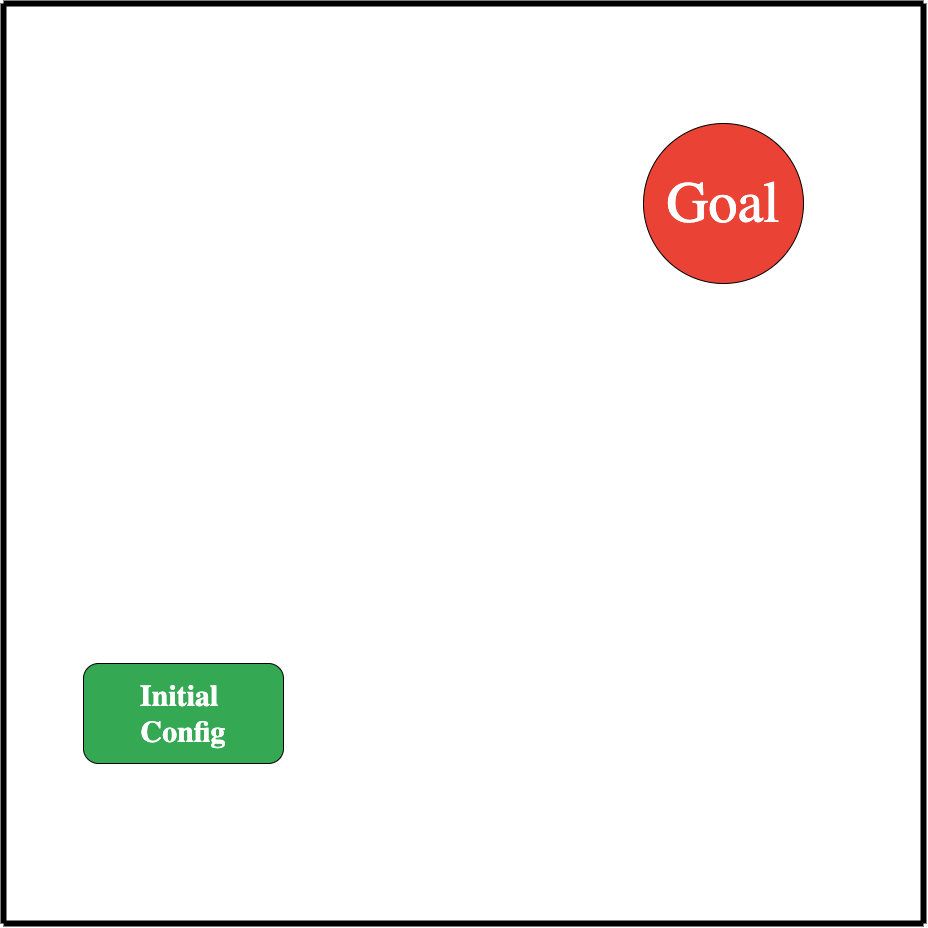
\includegraphics[draft=false,width=\linewidth]{chapters/chapter2/img/RRT_step_by_step-A.png}
    \caption{Graph $G$ contains only $q_{init}$ \newline}
    \label{subfig:rrt-step-by-step-A}
    \end{subfigure} &
    % 
    % Subfigure B
    \begin{subfigure}{0.45\textwidth}
    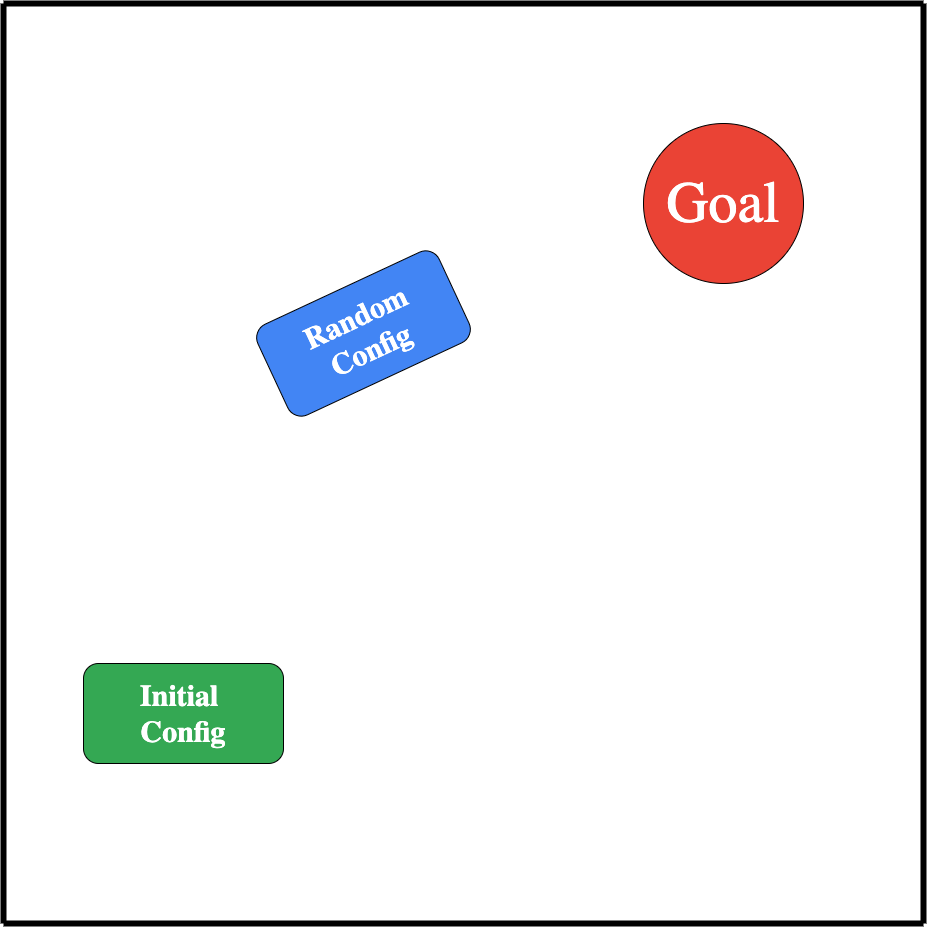
\includegraphics[draft=false,width=\linewidth]{chapters/chapter2/img/RRT_step_by_step-B.png}
    \caption{The first random configuration, $q_{rand}$, is generated}
    \label{subfig:rrt-step-by-step-B}
    \end{subfigure} \\ \\

    % Subfigure C
    \begin{subfigure}{0.45\textwidth}
    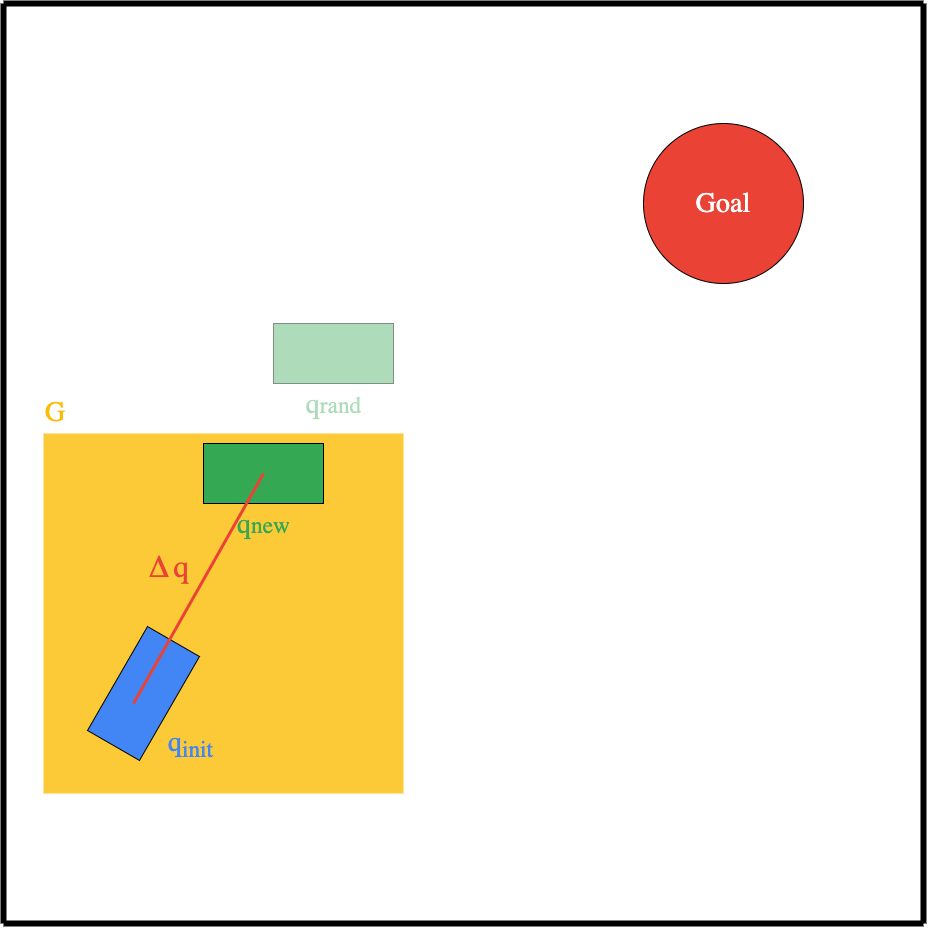
\includegraphics[draft=false,width=\linewidth]{chapters/chapter2/img/RRT_step_by_step-C.png}
    \caption{In first iteration, $q_{near} = q_{init}$. Distance between $q_{init}$ and $q_{rand}$ is greater than $\Delta q$, so $q_{new}$ is generated and added to $G$}
    \label{subfig:rrt-step-by-step-C}
    \end{subfigure} &
    % 
    % Subfigure D
    \begin{subfigure}{0.45\textwidth}
    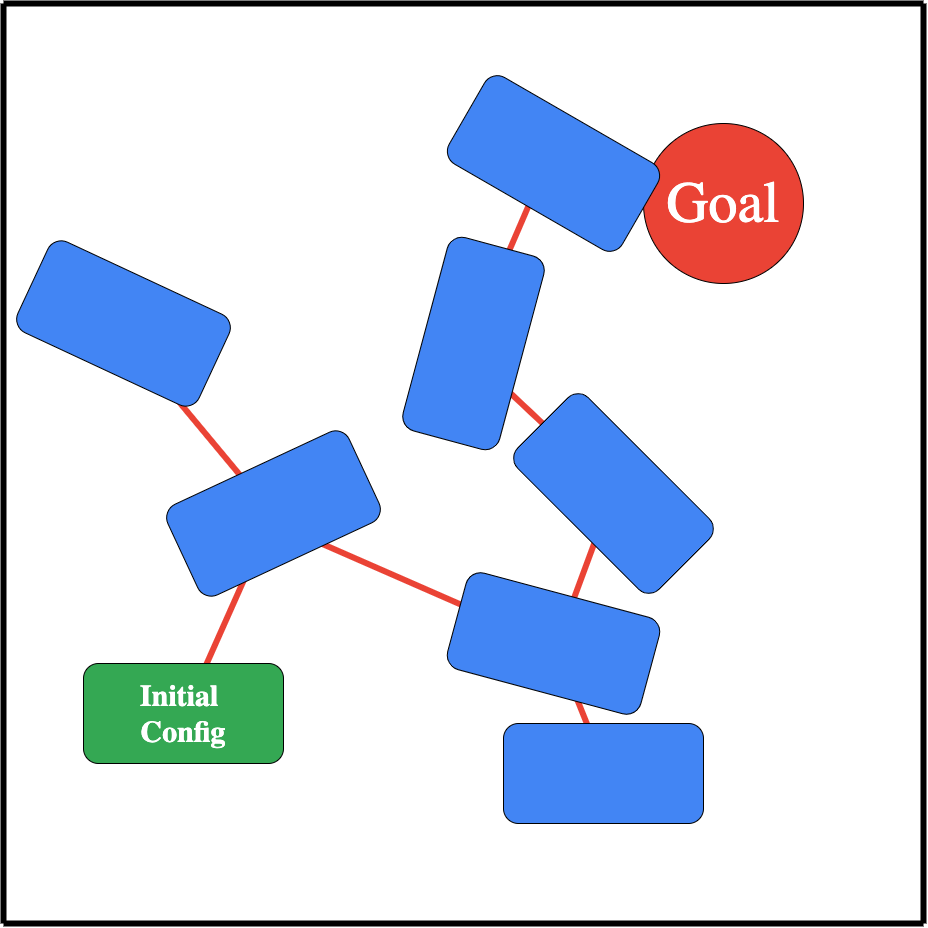
\includegraphics[draft=false,width=\linewidth]{chapters/chapter2/img/RRT_step_by_step-D.png}
    \caption{This is repeated $K$ times. For $G$, $K=10$, and the red line represents the edges between configurations}
    \label{subfig:rrt-step-by-step-D}
    \end{subfigure}

\end{tabular}
    
    % Caption and Label
    \caption{Step by step demonstration of \ac{RRT} Algorithm for 2D robot in 2D space}
    \label{fig:rrt-step-by-step}
\end{center}
\end{figure}

    \newpage % Delete

    The RRT Algorithm with Collision Detection can be seen in Algorthim \ref{algorithm:rrt_point}.
    % @Author: AnthonyKenny98
% @Date:   2020-02-22 16:15:38
% @Last Modified by:   AnthonyKenny98
% @Last Modified time: 2020-02-27 16:07:28

\bigskip
\begin{algorithm}[H]
    \caption{Rapidly-Exploring Random Tree with Collision Detection for Point Robot}
    \SetAlgoLined
    \SetArgSty{textnormal}
    \textbf{Inputs:} Space $S$ with obstacles \\ 
    \textbf{Output:} Collision free graph $G$ with $K$ nodes \& edges \\
        $G$.init()\;
        \For{$k = 1$ to $K$}{
            \While { !\text{pointCollision}($node_{new}$) } {
                $q_{rand} \leftarrow $ getRandomNode(); \\
                $q_{near} \leftarrow $ findNearestNode(); \\
                $q_{new} \leftarrow $ stepFromTo(); \\
            }
            $e_{new} \leftarrow $ newEdge($q_{near}, q_{new}$) \\
            \eIf{\text{!edgeCollision($e_{new}$)}} {
                $G$.addNode($q_{new}$); \\
                $G$.addEdge($e_{new}$);
            }{
                $k = k-1$;
            }
        }
\label{algorithm:rrt_point}
\end{algorithm}
\bigskip

\todo[inline]{Relook at above algorithm}

\subsection{Implementation}
    
    The project required an implementation of RRT that fulfilled the following criteria:

    \begin{enumerate}
        \item Implemented in C
        \item Modelled a drone as a point in a 3D space
        \item Was implemented in such a way that made it suitable for CPU execution analysis.
    \end{enumerate}

    The original intention was to find an existing implementation of RRT that could fulfill these requirements. Most open source implementations found online were in Python, and all those implemented in C were unsuitable\cite{RoboJackets2019}\cite{Planning2019}\cite{Sourishg2017}\cite{Vss2sn2019}, as they had extraneous \ac{GUI}s, reliance on external \ac{API}s, and other features that would distort analysis of algorithmic hotspots.

    As a result, it was neccesary to build a C implementation of RRT from the ground up. It can be found in this project's GitHub repository. It follows Algorithm \ref{algorithm:rrt} closely. For monitoring correctness, I build in an optional \ac{GUI} that shows the tree, starting node, and obstacles. 

    \subsubsection{Implementation in 2D}
    The first step was to implement RRT with a 2-Dimensional workspace. \todo[inline]{More detail}
    % @Author: AnthonyKenny98
% @Date:   2020-02-23 14:14:12
% @Last Modified by:   AnthonyKenny98
% @Last Modified time: 2020-03-01 08:06:12


\begin{figure}[H]
\begin{center}
\begin{tabular}{c  c}
    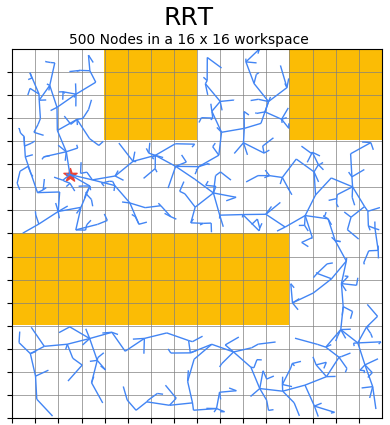
\includegraphics[width=0.45\linewidth]{chapters/chapter2/img/rrt_2d_1.png} & 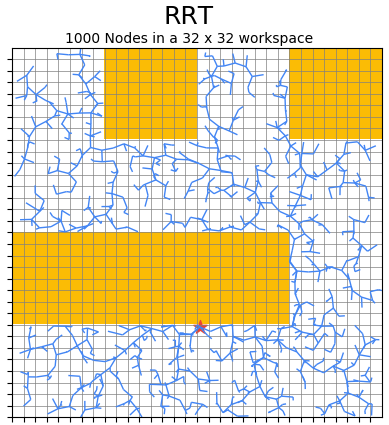
\includegraphics[width=0.45\linewidth]{chapters/chapter2/img/rrt_2d_2.png} \\
    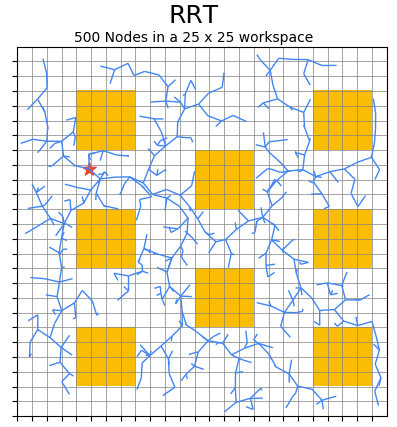
\includegraphics[width=0.45\linewidth]{chapters/chapter2/img/rrt_2d_3.png} & 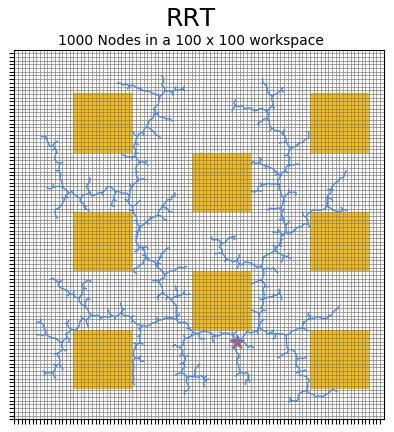
\includegraphics[width=0.45\linewidth]{chapters/chapter2/img/rrt_2d_4.png}
    \end{tabular}
    \caption{2D RRT Implementation shown by \ac{GUI}}
    \label{figure:2DrrtGui}
\end{center}
\end{figure}

    \subsubsection{Implementation in 3D}
    \todo[inline]{Describe implementation in 3D}
    % @Author: AnthonyKenny98
% @Date:   2020-02-23 14:14:12
% @Last Modified by:   AnthonyKenny98
% @Last Modified time: 2020-03-01 13:51:49


\begin{figure}[H]
\begin{center}
    \begin{tabular}{c  c}
    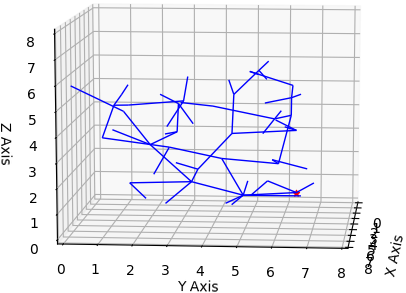
\includegraphics[width=0.45\linewidth]{chapters/chapter2/img/rrt_3d_1.png} & 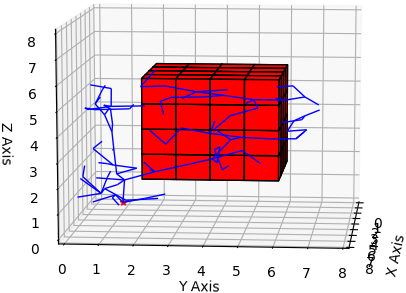
\includegraphics[width=0.45\linewidth]{chapters/chapter2/img/rrt_3d_2.png} \\
    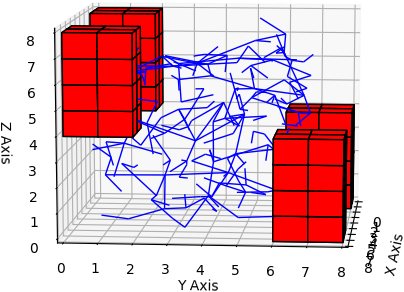
\includegraphics[width=0.45\linewidth]{chapters/chapter2/img/rrt_3d_3.png} & 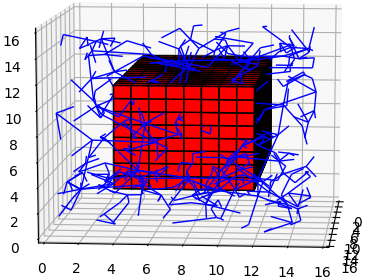
\includegraphics[width=0.45\linewidth]{chapters/chapter2/img/rrt_3d_4.png}
    \end{tabular}
    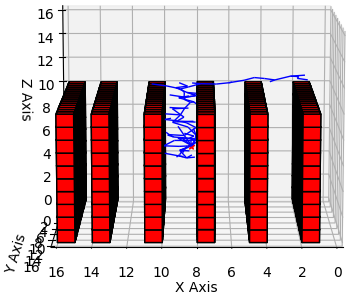
\includegraphics[width=0.45\linewidth]{chapters/chapter2/img/rrt_3d_5.png}
    \caption{3D RRT Implementation shown by \ac{GUI}}
    \label{figure:3DrrtGui}
\end{center}
\end{figure}

    


\subsection{Performance Analysis}
    To restate, the aim of this thesis is to design a computer processor with reduced execution time of motion planning algorithms, such as \ac{RRT}. As such, it is important to understand the elements of the algorithm that have the highest percentage of CPU execution time. To determine this, it was necessary to implement my own, naive but typical, \ac{RRT} in C. This program could then be compiled and analysed using a software performance profiling tool. With this, I could design experiments to determine the critical RRT functions (those occupying a majority of CPU time) and see how this varies given different paramaters.
    \todo[inline]{Introduction to purpose of analysis and methods of doing so. Something better than the above}

    \subsubsection{VTune Amplifier Analysis}
        VTune Amplifier performance profiler is an application for software performance analysis. It provides functionality to examine hotspots for CPU execution time through a top down analysis, shown below in Figure \ref{figure:VTuneTopDown}. As can be seen from the figure, the top down analysis tool shows the percentage of CPU time taken up by each function. I used this tool to profile the algorithm's performance as I changed certain parameters.
        \todo[inline]{Rewrite the above}
        % @Author: AnthonyKenny98
% @Date:   2020-02-23 14:33:19
% @Last Modified by:   AnthonyKenny98
% @Last Modified time: 2020-02-23 14:36:06

\begin{figure}[H]
\begin{center}
    \missingfigure[figwidth=\linewidth]{Screenshot of VTune Top Down Analysis (Maybe)}
    \caption{VTune Amplifier TopDown Analysis Example}
    \label{figure:VTuneTopDown}
\end{center}
\end{figure}

    \subsubsection{Internal Timing Analysis}

    \subsubsection{Comparison}